\section{Spannungswandler mit Ladungspumpen}

\begin{minipage}[c]{0.72\columnwidth}
    \begin{itemize}
        \item Ladung kann \textbf{nicht springen} und nicht vernichtet werden \\
            \textrightarrow\ Ladung wird umverteilt!
        \item Ladungspumpen sind billige, effiziente Spannungswandler (Wirkungsgrad $> 99 \, \%$ möglich)
    \end{itemize}
    
\end{minipage}
\hfill
\begin{minipage}[c]{0.25\columnwidth}
    $$ \boxed{ Q = C \cdot V} $$
\end{minipage}


\subsection{Grundprinzip Switched-Capacitor-Schaltungen (SC)}

\begin{minipage}[c]{0.28\columnwidth}
    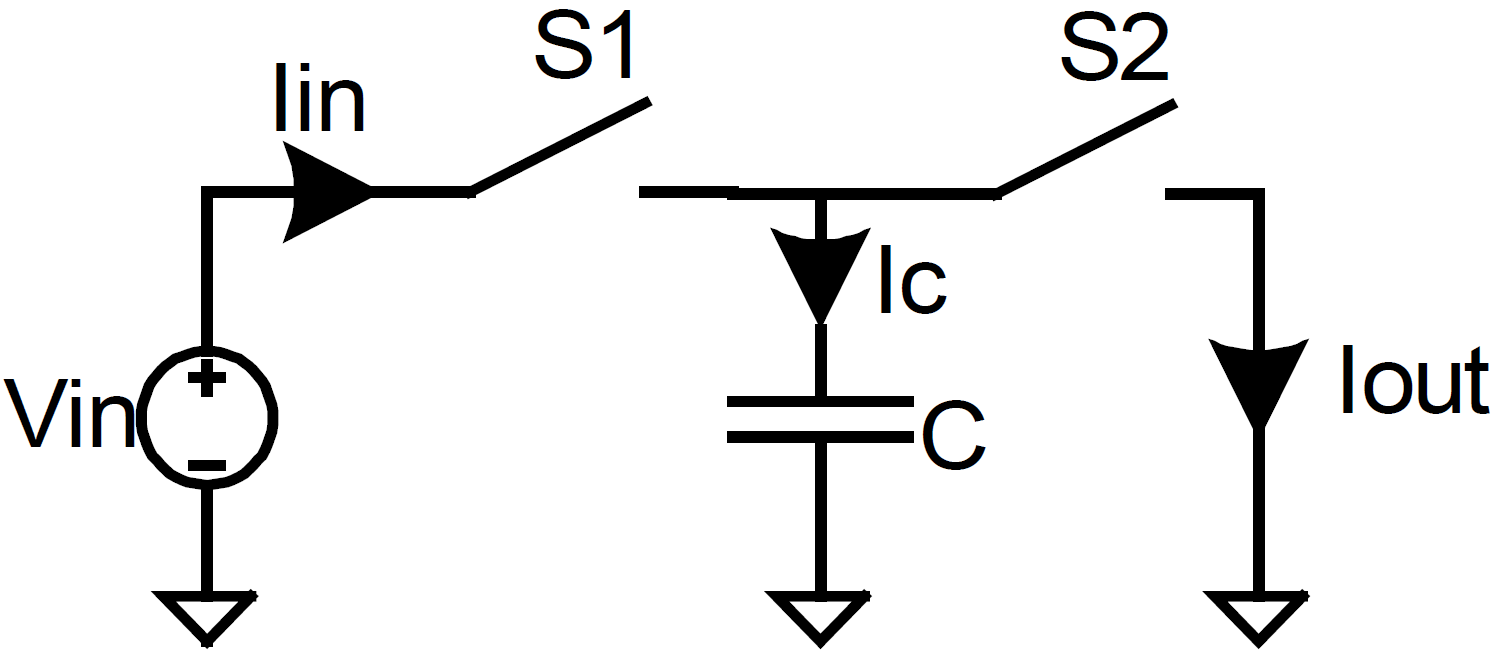
\includegraphics[width=\columnwidth]{images/grundprinzip_switched_capacitor_schaltung.png}
    \vspace{0.2cm}
    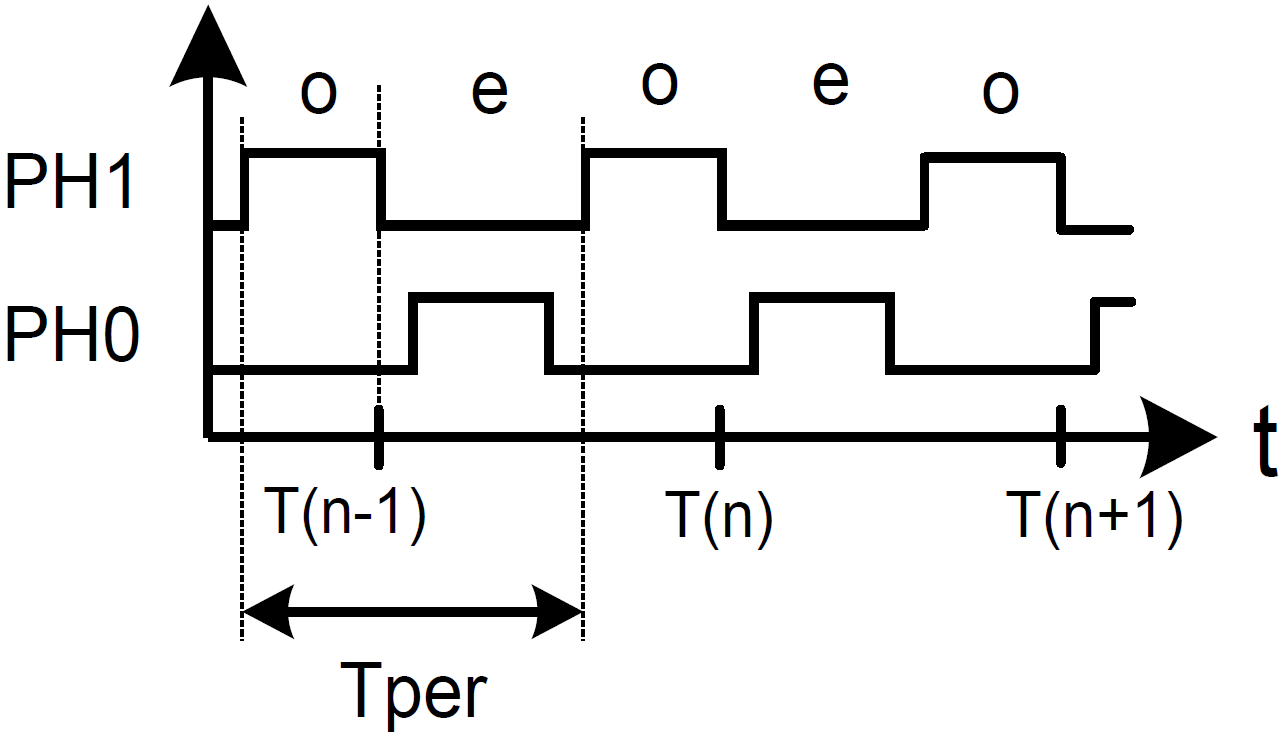
\includegraphics[width=\columnwidth]{images/grundprinzip_switched_capacitor_timing.png}
\end{minipage}
\hfill
\begin{minipage}[c]{0.7\columnwidth}
    \textbf{Hinweis:} $R_S$ entspricht dem Schalter-Widerstand \\
    Weiter gilt: $t^* = t - \frac{T}{2}$

    \begin{tabular}{ll@{}} 
        Phase PH1 (S1 geschl.)  & $I_{in} = I_C = \frac{V_{in}}{R_S} \cdot e^{\frac{t}{R_S \cdot C}} $ \\
        Phase PH2 (S2 geschl.)  & $I_C = - I_{out} = - \frac{V_{in}}{R_S} \cdot e^{\frac{t^*}{R_S \cdot C}}$ \\
        Durchschnittl. Strom    & $\overline{I_{out}} = \frac{\Delta Q}{T} =\frac{C}{T} \cdot V_{in}$ \\
    \end{tabular}

    Der 'switched capacitor' $C$ hat einen \textbf{äquivalenten Widerstand} $R_{eq} = \frac{T}{C} = \frac{1}{f \cdot C}$
\end{minipage}


\subsection{Grundprinzip Ladungspumpen}

\begin{minipage}[c]{0.5\columnwidth}
    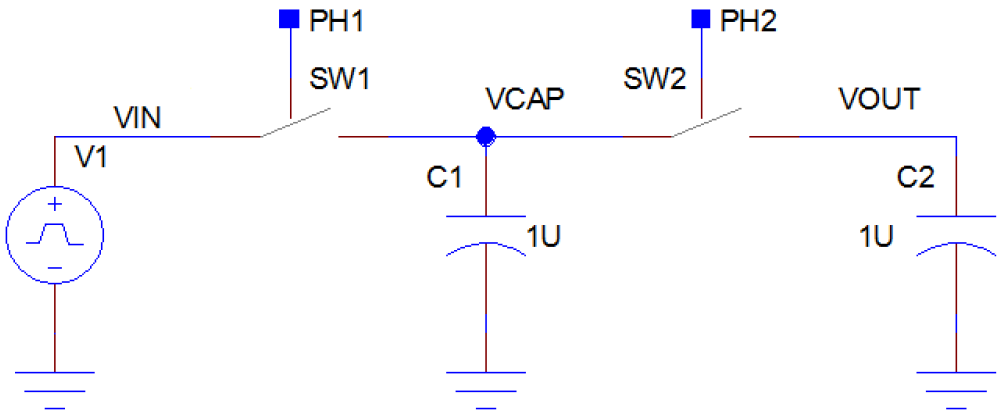
\includegraphics[width=\columnwidth]{images/grundprinzip_ladungspumpen.png} 
\end{minipage}
\hfill
\begin{minipage}[c]{0.33\columnwidth}
    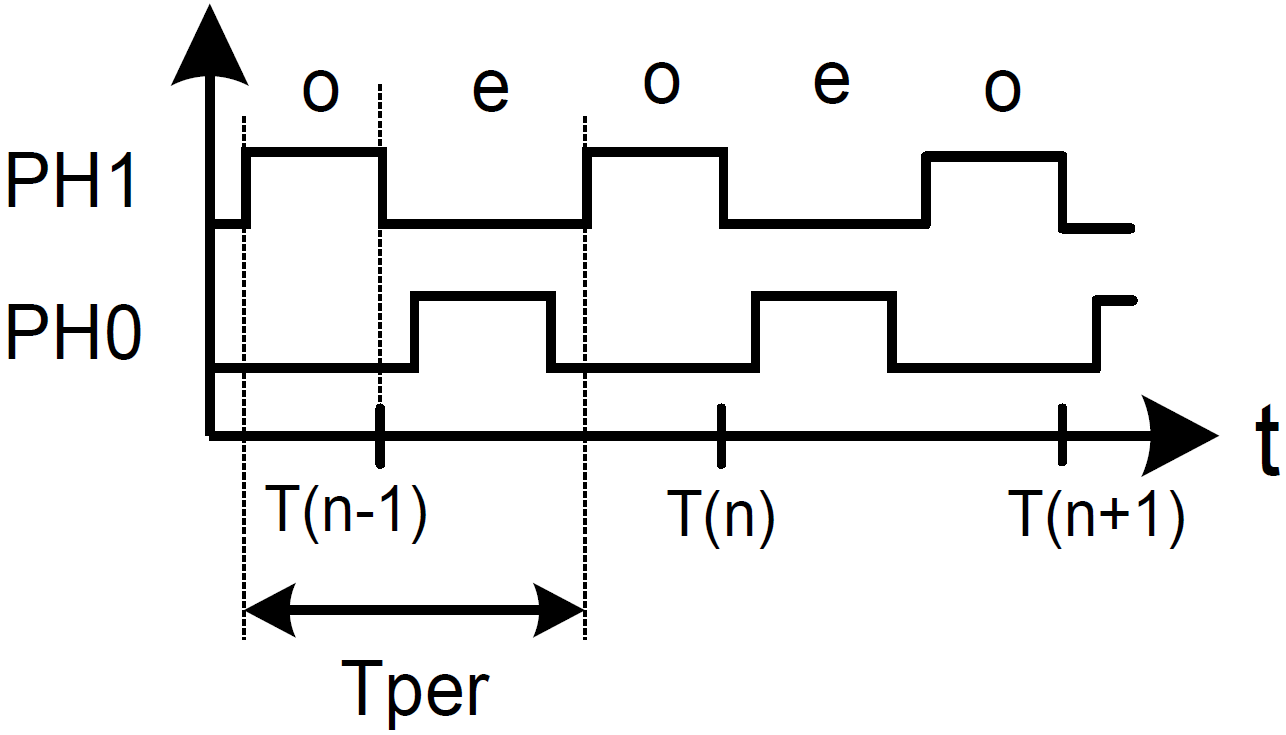
\includegraphics[width=\columnwidth]{images/grundprinzip_ladungspumpen_timing.png}
\end{minipage}

\vspace{0.2cm}
\textbf{Ausgangsspannung} $\bm{V_{out}}$ \textbf{nähert sich schrittweise exponentiell der Eingangsspannung an!} \\
Im ersten Zyklus ist $V_{out} = 0 \, \volt$

\begin{tabular}{ll@{}} 
    Phase PH1   & Kapazität $C_1$ wird auf $V_{in}$ geladen \\
                & $Q_1 = C_1 \cdot V_{in}$ und $Q_2 = C_2 \cdot V_{out}$ \\
    Phase PH2   & Ladung \textbf{verschiebt} sich von $C_1$ auf $C_2$, bis beide Kapazitäten \\
                & dieselbe Spannung aufweisen \\
                & $\cor{Q_{tot}} = Q_1 + Q_2 = C_1 \cdot V_{in} + C_2 \cdot V_{out} $ \\
                & \textrightarrow\ Neue Ausgangsspannung: $V_{out} = \frac{\cor{Q_{tot}}}{C_1 + C_2}$
\end{tabular}


\subsection{Allgemeine Funktionsweise geschaltete Kapazitäten}

\begin{minipage}[c]{0.46\columnwidth}
    \begin{center}
        \myul{Switched Capacitor $C_1$}
    \end{center}
    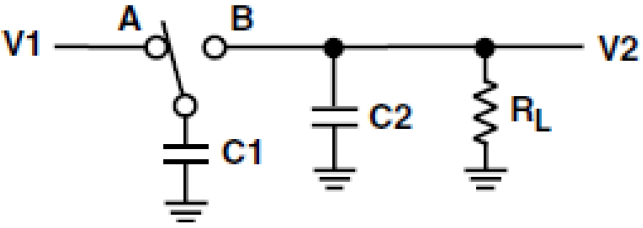
\includegraphics[width=\columnwidth]{images/sc_allgemein.png} 

    \begin{itemize}
        \item Strom fliesst in 'Paketen': \\
            $\Delta Q = C_1 \cdot \Delta V$ 
        \item Durchschnittlicher Strom proportional zu $C_1$, $\Delta V$ und Schaltfrequenz $f$
    \end{itemize}

\end{minipage}
\hfill
\begin{minipage}[c]{0.46\columnwidth}
    \begin{center}
        \myul{Ersatzschaltung mit $R_{eq}$}
    \end{center}
    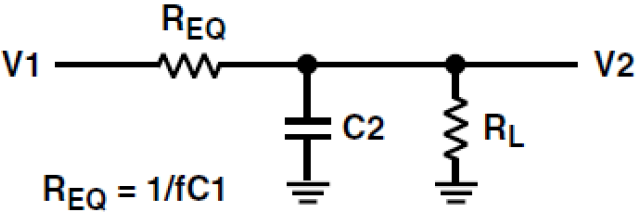
\includegraphics[width=\columnwidth]{images/rc_allgemein.png}

    \begin{itemize}
        \item Durchschnittlicher Strom proportional zu $\Delta V$ und $\frac{1}{R}$
        \item Geschaltetes $C_1$ bildet äquivalenten Widerstand $R_{eq} = \frac{1}{f \cdot C_1} = \frac{T}{C}$
    \end{itemize}
\end{minipage}

\vspace{0.2cm}
Für beide Schaltungen gilt, dass der \textbf{finale Wert der Ausgangsspannung} $V_{out} = V_2$ durch den 
\textbf{Spannungsteiler} von $R_L$ und $R_{eq}$ bestimmt wird:

\begin{minipage}[c]{0.48\columnwidth}
    $$ \boxed{ V_{out} = V_{in} \cdot \frac{R_L}{R_{eq} + R_L} } $$
\end{minipage}
\hfill
\begin{minipage}[c]{0.48\columnwidth}
    $$ \boxed{ I = \frac{V_1 - V_2}{R_{eq}} } $$
\end{minipage}


\subsection{Spannungsinversion mit Switched Capacitors}

\begin{center}
    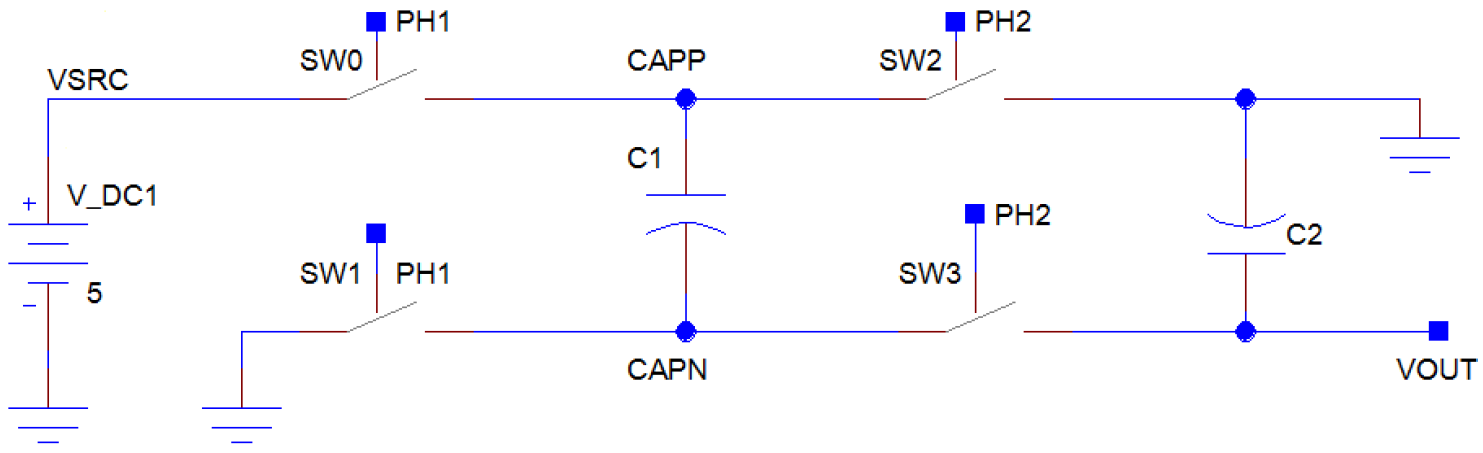
\includegraphics[width=0.75\columnwidth]{images/spannungsinverter.png}
\end{center}

\textbf{Ausgangsspannung} $\bm{V_{out}}$ \textbf{nähert sich schrittweise exponentiell $\bm{-V_{SRC}}$ an!} \\
Im ersten Zyklus ist $V_{out} = 0 \, \volt$

\begin{tabular}{ll@{}} 
    Phase PH1   & Kapazität $C_1$ wird auf $V_{SRC}$ geladen \\
                & $Q_1 = C_1 \cdot V_{SRC}$ und $Q_2 = C_2 \cdot V_{out}$ \\
    Phase PH2   & Positiver Anschluss von $C_1$ wird mit GND verbunden \\
                & \textrightarrow\ Negativer Anschluss von $C_1$ auf Potential $- V_{SRC}$ \\
                & $\cor{Q_{tot}} = Q_2 - Q_1 = C_2 \cdot V_{out} - C_1 \cdot V_{SRC}$ \\
                & \textrightarrow\ Neue Ausgangsspannung: $V_{out} = \frac{\cor{Q_{tot}}}{C_1 + C_2}$\\   % // CHECK if this is correct
\end{tabular}
\vspace{0.2cm}
Für  $C_1 = C_2$ ändert sich die Ausgangsspannung $V_{out}$ folgendermassen:
$$ V_{out} = (- \frac{1}{2}, - \frac{3}{4}, - \frac{7}{8} \cdots -1) \cdot V_{SRC} $$


\subsection{Spanungsverdoppler mit Switched Capacitors}

\begin{center}
    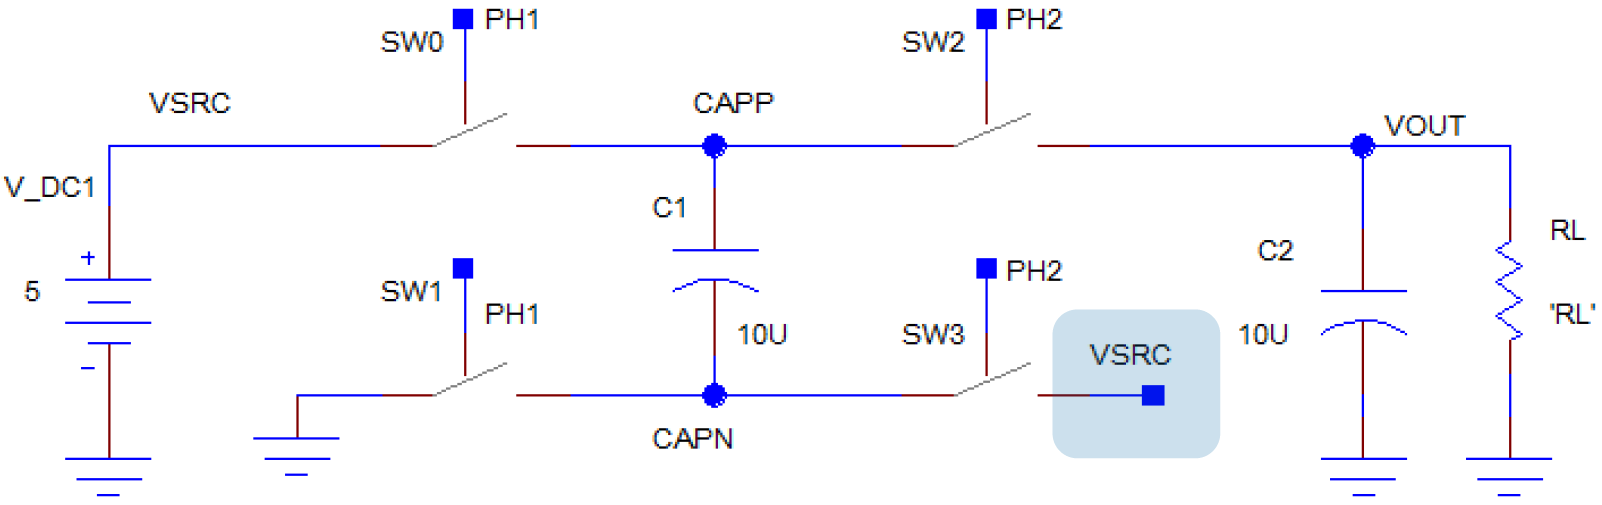
\includegraphics[width=0.75\columnwidth]{images/spannungsverdoppler.png}
\end{center}

\begin{itemize}
    \item PH1: $C_1$ wird auf Eingangsspannung $V_{in}$ aufgeladen
    \item PH2: Negativer Anschluss CAPN wird mit $V_{SRC}$ verbunden \textrightarrow\ Positiver Anschluss $C_1$ springt auf $2 \cdot V_{SRC} $
    \item Ladung teilt sich zwischen $C_1$ und $C_2$ auf, sodass $V_{out}$ schrittweise ansteigt 
\end{itemize}


\subsection{Dickson Charge Pump (Spannungsvervielfacher)}

\begin{minipage}[c]{0.55\columnwidth}
    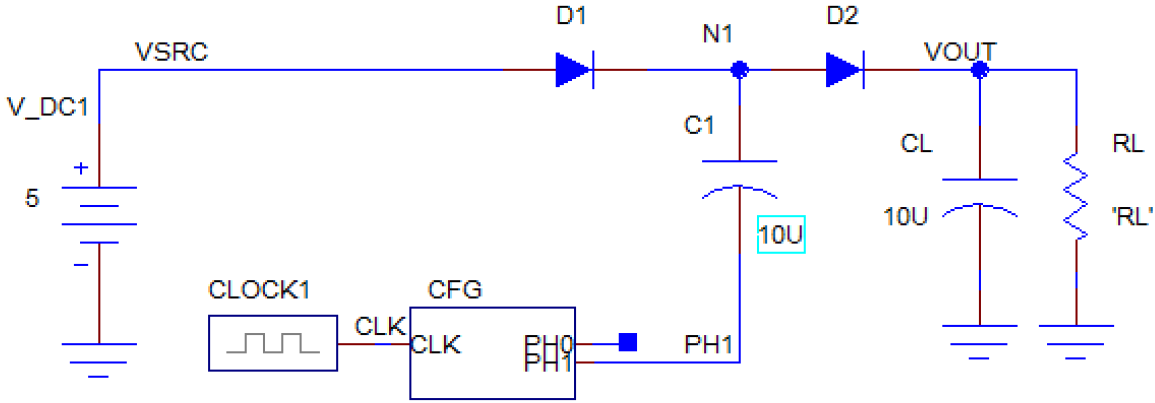
\includegraphics[width=\columnwidth]{images/dickson_charge_pump.png}
\end{minipage}
\hfill
\begin{minipage}[c]{0.43\columnwidth}
    \begin{itemize}
        \item Mehrstufige Spannungsvervielfacher (hier: einstufig)
        \item Anzahl Dioden $n$ 
        \item Kaskadierung möglich
    \end{itemize}
    $$ \boxed{ V_{out} = n \cdot (V_{SRC} - V_D) } $$
\end{minipage}


\subsubsection{Mehrstufige Dickson Charge Pump}

\begin{minipage}[c]{0.5\columnwidth}
    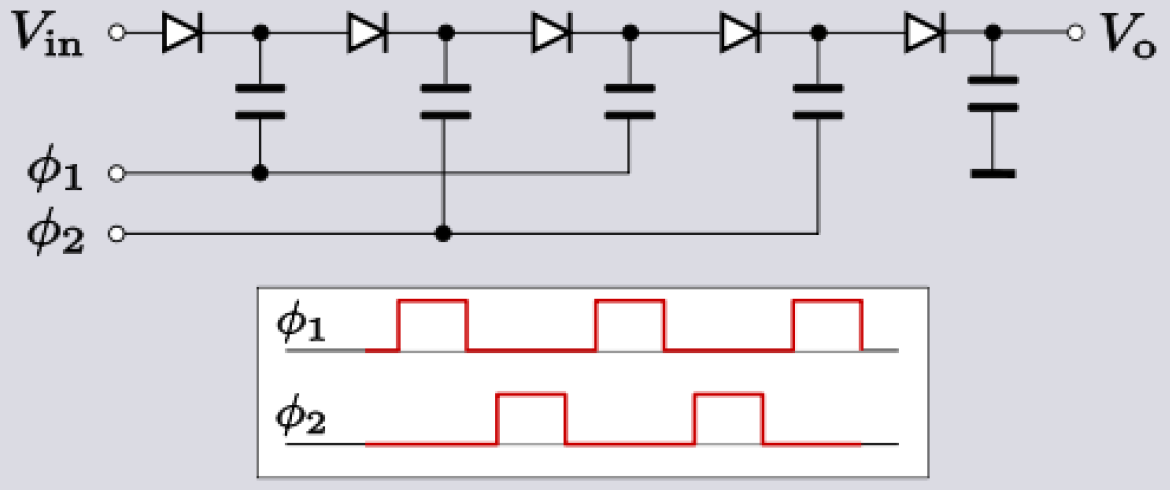
\includegraphics[width=\columnwidth]{images/dickson_charge_pump_mehrstufig.png}
\end{minipage}
\hfill
\begin{minipage}[c]{0.48\columnwidth}
    \begin{itemize}
        \item Mehrstufige Spannungsvervielfacher (hier: $n = 5$)
    \end{itemize}

    $$ \boxed{ V_{out} = n \cdot (V_{SRC} - V_D) } $$
\end{minipage}